\chapter{既存のシミュレータによる表現} \label{background}

本章では、斜方投射の例を通して既存のシミュレータである PhET~\cite{perkins_phet_2006} の表現方法ついて説明する。

\section{斜方投射}
斜方投射は、次のような現象である。
\begin{quote}
ある物体を原点から時刻 $t=0$ に、$x$ 軸方向の初速 $v_{0x}$ 、$y$ 軸方向の初速 $v_{0y}$ で投げる。このとき、重力加速度の大きさを $g$ とすると、物体は次のような軌道を描く。
\begin{equation}
\left\{
\begin{aligned}
  x &= v_{0x} t \\
  y &= v_{0y} t - \dfrac{1}{2}gt^2 \\
\end{aligned}
\right.
\end{equation} \label{斜方投射連立}
\end{quote}

\begin{figure}[H]
\centering
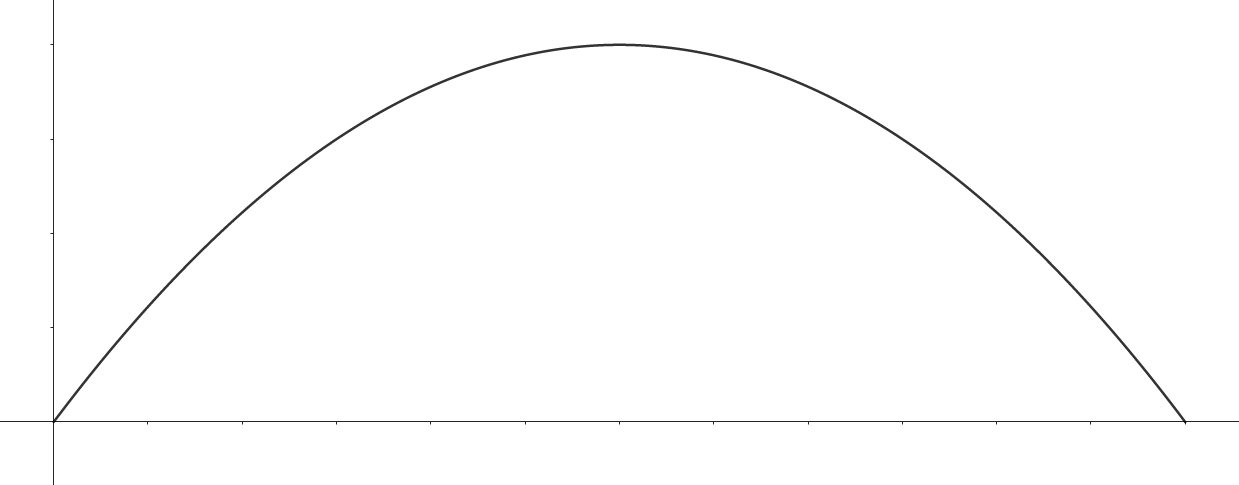
\includegraphics[width=0.9\linewidth]{figure/curve.png}
\end{figure}

\section{PhET による斜方投射の表現}

PhET (Physics Education Technology) は、コロラド大学ボルダー校によるプロジェクトで、物理学の教育に活用できるシミュレーションの作成を目標としている。2023年2月現在、ウェブサイト\footnote{\url{https://phet.colorado.edu}}上では50以上のシミュレーションが公開されている。また、物理学のみならず化学・数学・生物学・地球科学などのシミュレーションも公開されている。PhET を用いることで、実際の実験を行うのと同様な教育効果が得られる~\cite{ajredini_real_2014}。

PhET を用いた授業では、以下のような順番で授業を構成することが推奨されている\footnote{\url{https://phet.colorado.edu/files/guides/UG_Phys_Guide-Lecture-Overview_en.pdf}}。
\begin{enumerate}
  \item シナリオを提示する。
  \item 学習者が各自で法則について予想する。
  \item 学習者間でディスカッションを行い、予測を修正する。
  \item 教育者が学習者の予測や推論を引き出す。
  \item 教育者がシミュレーションを用いて実験を行う。
  \item 学習者は結果を記録し、予測とどう違うかを記録する。
  \item 学習者全体でディスカッションを行う。推論に重点を置く。
\end{enumerate}

図~\ref{numeral_based}は、PhET 上で斜方投射のシミュレーションを行った様子である。大砲から砲弾が射出されるという設定で表現されている。学習者は、初速度や砲弾の質量、仰角などを数値で指定することができ、軌道や着弾点を測定することができる。

このシミュレーションを通して、学習者は斜方投射の運動を観察することができる。一方で、シミュレーションを作成するのは教育者である。そのため、この軌道や着弾点の位置が具体的にどのような方程式に基づいて計算されたものなのかはわからず、式(\ref{斜方投射連立})が現実の現象と一致しているという実感は得にくいと考えられる。
